\section{Projected Sensitivity}
\par
The determination of the LZ sensitivity to EFT recoils is perform analogously to \cite{LZ_projected_sensitivity_paper_ref} but with 

\subsection{Background Models}
\par
Our background model is based upon the components that we introduced in \autoref{sec:lz_detector}, but limited to only taking the largest contributions.
Leaving us with 11 components shown in \autoref{tab:projected_lz_backgrounds}.


\subsection{Simulations}
\par
The simulations used to produce the PDFs for the PLR originate from those used in \cite{LZ_projected_sensitivity_paper_ref} where an energy deposit only approach was adopted based upon a detector response model for which the author takes no credit and so only the essential information is detailed here.
A more complete description of the simulation framework and detector response can be found in the following Refs. \cite{lz_simulations_ref,theresafruth_thesis_ref}.
\par
In order to determine the detector response, a set of simulations were performed in the standard fashion; where an energy deposit in xenon is translated into scintillation photons and ionisation electrons using NEST \cite{nest_1_ref,nest_2_ref}.
These were then propagated until eventual detection (or not) at the PMT faces where the PMT response is then incorporated.
The resultant sum of these responses give us the S1 and S2 pulse sizes from which the detector response is made from, describing the size of the S1 and S2 for a given recoil.
Our detector is then described by a finite number of parameters given \autoref{tab:projected_sensitivity_detector_parameters} and the response in S1$_c$ and S2$_c$ for a NR events is shown in \autoref{fig:projected_detector_model_response_for_flat_nr}.
When it comes time to generate the PDFs required for our PLR we can simply use the differential scattering rate per recoil energy.
\begin{table}[]
    \centering
    \begin{tabular}{c|c}
        Parameter   & Value  \\ \hline
        $g_{1}$     & 0.119 \\
        $g_{2}$     & 79.1  \\
        Drift field & 310 Vcm$^{-1}$ \\
        electron lifetime & 850 $\mu$s
    \end{tabular}
    \caption{Key detector parameters for the LXe-TPC parameters in the projected detector performance case.}
    \label{tab:projected_sensitivity_detector_parameters}
\end{table}
\begin{figure}[!htbp]%
\centering
    \begin{tikzpicture}
    \centering
        \begin{groupplot}[view={0}{90},
            group style = {group size = 2 by 1,
            horizontal sep=0.6cm}]
            \nextgroupplot[
            width=0.48\textwidth, height=8cm,
            xlabel={Recoil Energy [keV$_{NR}$]},
            ylabel={S1$_{c}$ [phd]},
            mark size=0pt,
            xmin=0, xmax=300,
            ymin=0, ymax=600]

            \addplot[yellow, name path = psig2] table[x=energy, y=psig2]
                      {Data/HENR/Projected_Sensitivity/data_cuts/s1_vs_recoil.dat};
            \addplot[yellow, name path = nsig2] table[x=energy, y=nsig2]
                      {Data/HENR/Projected_Sensitivity/data_cuts/s1_vs_recoil.dat};
            
            \addplot[green, name path = psig1] table[x=energy, y=psig1]
                      {Data/HENR/Projected_Sensitivity/data_cuts/s1_vs_recoil.dat};
            \addplot[green, name path = nsig1] table[x=energy, y=nsig1]
                      {Data/HENR/Projected_Sensitivity/data_cuts/s1_vs_recoil.dat};
                      
            \addplot[yellow, forget plot] fill between[of=nsig2 and psig2]; 
            \addplot[green, forget plot] fill between[of=nsig1 and psig1];
            
            \addplot[black] table[x=energy, y=mean]
                    {Data/HENR/Projected_Sensitivity/data_cuts/s1_vs_recoil.dat};
            
            \addplot[blue, dashed] coordinates { (0,500)  (325,500)};
            \addplot[black, dashed] coordinates { (278,0)  (278,700)};
                  
            \nextgroupplot[
            width=0.48\textwidth, height=8cm,
            xlabel={Recoil Energy [keV$_{NR}$]},
            ylabel={log$_{10}$(S2$_{c}$ [phd])},
            yticklabel pos=right,
            mark size=0pt,
            xmin=0, xmax=300,
            ymin=2.0, ymax=5.0]
            
            \addplot[yellow, name path = psig2] table[x=energy, y=psig2]
                      {Data/HENR/Projected_Sensitivity/data_cuts/logs2_vs_recoil.dat};
            \addplot[yellow, name path = nsig2] table[x=energy, y=nsig2]
                      {Data/HENR/Projected_Sensitivity/data_cuts/logs2_vs_recoil.dat};
            \addplot[yellow, forget plot] fill between[of=nsig2 and psig2];          
            
            \addplot[green, name path = psig1] table[x=energy, y=psig1]
                      {Data/HENR/Projected_Sensitivity/data_cuts/logs2_vs_recoil.dat};
            \addplot[green, name path = nsig1] table[x=energy, y=nsig1]
                      {Data/HENR/Projected_Sensitivity/data_cuts/logs2_vs_recoil.dat};
            \addplot[green, forget plot] fill between[of=nsig1 and psig1];
            
            \addplot[black] table[x=energy, y=mean]
                    {Data/HENR/Projected_Sensitivity/data_cuts/logs2_vs_recoil.dat};
                    
            \addplot[black, dashed] coordinates { (278,2)  (278,5)};
        
        \end{groupplot}
    \end{tikzpicture}
    \caption{Detector response in S1 (\textbf{Left}) and S2 (\textbf{Right}) space for a given recoil in the LZ detector assuming the projected detector parameters.
             The values have been extrapolated from simulations of a flat NR spectrum.
    }
    \label{fig:projected_detector_model_response_for_flat_nr}
\end{figure}


\subsection{Signal Model}
\par
The package used here is DMFormFactor v6.0 as was the choice for both LUX and XENON collaboration results\footnote{At the time of writing this is the newest public release. However these is a newer version which uses updated form factors which was used in \cite{pandax_2_eft_ref}.}.
The Standard Halo Model parameters used to describe the dark matter are summarised in \autoref{tab:DMFormFactor_parameters}.
\begin{table}[]
    \centering
    \begin{tabular}{c|c}
        Parameter         & Value  \\ \hline
        $\nu_0$           & 220$km s^{-1}$ \\
        $\nu_{esc}$       & 544$km s^{-1}$ \\
        $\rho_{\chi}$     & 0.3 $GeV/cm^{3}$ \\
        $|\nu_E|$         & 245 $km s^{-1}$ 
    \end{tabular}
    \caption{DMFormFactor parameters used for the standard halo model. CITE XXX}
    \label{tab:DMFormFactor_parameters}
\end{table}
To improve the realism of the recoil and to maintain consistency with previous experiments the natural abundance of Xe isotopes were folded in.
Each operator was generated out to 1000 keV and in the isoscalar basis and a selection of the resultant differential rates are shown in \autoref{fig:HENR_Spin_Recoil_Spectrum}.
Each Operator was performed for a WIMP mass of [5, 7, 10, 12, 14, 21, 33, 50, 100, 200, 400, 1000, 4000] GeV.

\begin{figure}[!htbp]%
\centering
\begin{tikzpicture}
\centering
  \begin{groupplot}[view={0}{90},
    group style = {group size = 1 by 3}]
    \iffalse
    \nextgroupplot[
    xlabel=Recoil Energy (keV),
    ylabel=Differential Rate (kg/day/keV),
    legend pos=north east,
    mark size=0pt,
    xmin=1, xmax=400, xmode=log,
    ymin=1e-14, ymax=1e3, ymode=log]
    \addplot table {Data/HENR/Projected_Sensitivity/Signal/Recoils/dRdEr_EFT_O01s_m50GeV_0.dat};
    \addplot table {Data/HENR/Projected_Sensitivity/Signal/Recoils/dRdEr_EFT_O11s_m50GeV_0.dat};       
    \legend{$\Operator$1s, $\Operator$11s};
    \fi
    \nextgroupplot[
    xlabel=Recoil Energy (keV),
    ylabel=Differential Rate (kg/day/keV),
    legend pos=north east,
    mark size=0pt,
    xmin=1, xmax=400, xmode=log,
    ymin=1e-14, ymax=1e3, ymode=log,
    cycle list name=color list]
    \addplot table {Data/HENR/Projected_Sensitivity/Signal/Recoils/dRdEr_EFT_O04s_m50GeV_0.dat};
    \addplot table {Data/HENR/Projected_Sensitivity/Signal/Recoils/dRdEr_EFT_O06s_m50GeV_0.dat};     
    \addplot table {Data/HENR/Projected_Sensitivity/Signal/Recoils/dRdEr_EFT_O07s_m50GeV_0.dat};
    \addplot table {Data/HENR/Projected_Sensitivity/Signal/Recoils/dRdEr_EFT_O09s_m50GeV_0.dat};
    \addplot table {Data/HENR/Projected_Sensitivity/Signal/Recoils/dRdEr_EFT_O10s_m50GeV_0.dat};
    \addplot table {Data/HENR/Projected_Sensitivity/Signal/Recoils/dRdEr_EFT_O14s_m50GeV_0.dat};
    \legend{$\Operator$4s, $\Operator$6s, $\Operator$7s, $\Operator$9s, $\Operator$10s, $\Operator$14s};
    \iffalse
    \nextgroupplot[
    xlabel=Recoil Energy (keV),
    ylabel=Differential Rate (kg/day/keV),
    legend pos=north east,
    mark size=0pt,
    xmin=1, xmax=400, xmode=log,
    ymin=1e-14, ymax=1e3, ymode=log]
    \addplot table {Data/HENR/Projected_Sensitivity/Signal/Recoils/dRdEr_EFT_O03s_m50GeV_0.dat};
    \addplot table {Data/HENR/Projected_Sensitivity/Signal/Recoils/dRdEr_EFT_O05s_m50GeV_0.dat};
    \addplot table {Data/HENR/Projected_Sensitivity/Signal/Recoils/dRdEr_EFT_O08s_m50GeV_0.dat};
    \addplot table {Data/HENR/Projected_Sensitivity/Signal/Recoils/dRdEr_EFT_O12s_m50GeV_0.dat};
    \addplot table {Data/HENR/Projected_Sensitivity/Signal/Recoils/dRdEr_EFT_O13s_m50GeV_0.dat};
    \addplot table {Data/HENR/Projected_Sensitivity/Signal/Recoils/dRdEr_EFT_O15s_m50GeV_0.dat};       
    \legend{$\Operator$3s, $\Operator$5s, $\Operator$8s, $\Operator$12s, $\Operator$13s, $\Operator$15s};
    \fi
  \end{groupplot}
\end{tikzpicture}
\caption{Differential recoil spectra for the fourteen non-relativistic EFT WIMP-nucleon operators with a WIMP mass of 50 GeV/c$^2$.
         \textbf{Top:} spin-independent \textbf{Middle:} spin-dependent \textbf{Bottom:} novel }
\label{fig:HENR_recoil_spectra_m50}
\end{figure}


\begin{figure}[!htbp]%
\centering
\begin{tikzpicture}
\centering
  \begin{groupplot}[view={0}{90},
    group style = {group size = 1 by 3}]
    
    \nextgroupplot[
    xlabel=Recoil Energy (keV),
    ylabel=Differential Rate (kg/day/keV),
    legend pos=north east,
    mark size=0pt,
    xmin=1, xmax=400, xmode=log,
    ymin=1e-14, ymax=1e3, ymode=log]
    \addplot table {Data/HENR/Projected_Sensitivity/Signal/Recoils/dRdEr_EFT_O01s_m33GeV_0.dat};
    \addplot table {Data/HENR/Projected_Sensitivity/Signal/Recoils/dRdEr_EFT_O11s_m33GeV_0.dat};       
    \legend{$\Operator$1s, $\Operator$11s};
    \iffalse
    \nextgroupplot[
    xlabel=Recoil Energy (keV),
    ylabel=Differential Rate (kg/day/keV),
    legend pos=north east,
    mark size=0pt,
    xmin=1, xmax=400, xmode=log,
    ymin=1e-14, ymax=1e3, ymode=log,
    cycle list name=color list]
    \addplot table {Data/HENR/Projected_Sensitivity/Signal/Recoils/dRdEr_EFT_O04s_m1000GeV_0.dat};
    \addplot table {Data/HENR/Projected_Sensitivity/Signal/Recoils/dRdEr_EFT_O06s_m1000GeV_0.dat};     
    \addplot table {Data/HENR/Projected_Sensitivity/Signal/Recoils/dRdEr_EFT_O07s_m1000GeV_0.dat};
    \addplot table {Data/HENR/Projected_Sensitivity/Signal/Recoils/dRdEr_EFT_O09s_m1000GeV_0.dat};
    \addplot table {Data/HENR/Projected_Sensitivity/Signal/Recoils/dRdEr_EFT_O10s_m1000GeV_0.dat};
    \addplot table {Data/HENR/Projected_Sensitivity/Signal/Recoils/dRdEr_EFT_O14s_m1000GeV_0.dat};
    \legend{$\Operator$4s, $\Operator$6s, $\Operator$7s, $\Operator$9s, $\Operator$10s, $\Operator$14s};
    
    \nextgroupplot[
    xlabel=Recoil Energy (keV),
    ylabel=Differential Rate (kg/day/keV),
    legend pos=north east,
    mark size=0pt,
    xmin=1, xmax=400, xmode=log,
    ymin=1e-14, ymax=1e3, ymode=log]
    \addplot table {Data/HENR/Projected_Sensitivity/Signal/Recoils/dRdEr_EFT_O03s_m1000GeV_0.dat};
    \addplot table {Data/HENR/Projected_Sensitivity/Signal/Recoils/dRdEr_EFT_O05s_m1000GeV_0.dat};
    \addplot table {Data/HENR/Projected_Sensitivity/Signal/Recoils/dRdEr_EFT_O08s_m1000GeV_0.dat};
    \addplot table {Data/HENR/Projected_Sensitivity/Signal/Recoils/dRdEr_EFT_O12s_m1000GeV_0.dat};
    \addplot table {Data/HENR/Projected_Sensitivity/Signal/Recoils/dRdEr_EFT_O13s_m1000GeV_0.dat};
    \addplot table {Data/HENR/Projected_Sensitivity/Signal/Recoils/dRdEr_EFT_O15s_m1000GeV_0.dat};       
    \legend{$\Operator$3s, $\Operator$5s, $\Operator$8s, $\Operator$12s, $\Operator$13s, $\Operator$15s};
    \fi
  \end{groupplot}
\end{tikzpicture}
\caption{Differential recoil spectra for the fourteen non-relativistic EFT WIMP-nucleon operators with a WIMP mass of 1000 GeV/c$^2$.
         \textbf{Top:} spin-independent \textbf{Middle:} spin-dependent \textbf{Bottom:} novel }
\label{fig:HENR_recoil_spectra_m1000}
\end{figure}

\iffalse

\begin{figure}[!htbp]%
\centering
\begin{tikzpicture}
\centering
  \begin{groupplot}[view={0}{90},
    group style = {group size = 3 by 1}]
    \nextgroupplot[
    xlabel=Recoil Energy (keV),
    ylabel=Differential Rate (kg/day/keV),
    legend pos=north east,
    mark size=0pt,
    xmin=1, xmax=400, xmode=log,
    ymin=1e-14, ymax=1e3, ymode=log]
    \foreach \henrop in \roguerecoiloperators{
                \addplot 
                    table
                    %{Data/HENR/Signal/Recoils/dRdEr_EFT_O01s_m5GeV_0.txt};
                    {Data/HENR/Projected_Sensitivity/Signal/Recoils/dRdEr_EFT_O\henrop_m5GeV_0.dat};
            }
    \nextgroupplot[
    xlabel=Recoil Energy (keV),
    legend pos=north east,
    mark size=0pt,
    xmin=1, xmax=400, xmode=log,
    ymin=1e-14, ymax=1e3, ymode=log]
    \foreach \henrop in \roguerecoiloperators{
                \addplot
                    table
                    %{Data/HENR/Signal/Recoils/dRdEr_EFT_O01s_m5GeV_0.txt};
                    {Data/HENR/Projected_Sensitivity/Signal/Recoils/dRdEr_EFT_O\henrop_m5GeV_0.dat};
            }
  \end{groupplot}
\end{tikzpicture}
\caption{Literal Aids
\textbf{Left:} $Gd^{156}$ de-excitation path.
\textbf{Right:} $Gd^{158}$ de-excitation path.
}
\label{fig:HENR_NotSpin_Recoil_Spectrum}
\end{figure}


\begin{figure}[!htbp]%
\centering
\begin{tikzpicture}
\centering
  \begin{groupplot}[view={0}{90},
    group style = {group size = 2 by 1}]
    \nextgroupplot[
    xlabel=Recoil Energy (keV),
    ylabel=Differential Rate (kg/day/keV),
    legend pos=north east,
    mark size=0pt,
    xmin=1, xmax=400, xmode=log,
    ymin=1e-14, ymax=1e3, ymode=log]
    \foreach \henrop in \spinrecoiloperators{
                \addplot 
                    table
                    %{Data/HENR/Signal/Recoils/dRdEr_EFT_O01s_m5GeV_0.txt};
                    {Data/HENR/Projected_Sensitivity/Signal/Recoils/dRdEr_EFT_O\henrop_m5GeV_0.dat};
            }
    \nextgroupplot[
    xlabel=Recoil Energy (keV),
    legend pos=north east,
    mark size=0pt,
    xmin=1, xmax=400, xmode=log,
    ymin=1e-14, ymax=1e3, ymode=log]
    \foreach \henrop in \spinrecoiloperators{
                \addplot
                    table
                    %{Data/HENR/Signal/Recoils/dRdEr_EFT_O01s_m5GeV_0.txt};
                    {Data/HENR/Projected_Sensitivity/Signal/Recoils/dRdEr_EFT_O\henrop_m21GeV_0.dat};
            }
  \end{groupplot}
\end{tikzpicture}
\caption{Literal Aids
\textbf{Left:} $Gd^{156}$ de-excitation path.
\textbf{Right:} $Gd^{158}$ de-excitation path.
}
\label{fig:HENR_Spin_Recoil_Spectrum}
\end{figure}

\begin{figure}[!htbp]%
\centering
\begin{tikzpicture}
\centering
  \begin{groupplot}[view={0}{90},
    group style = {group size = 2 by 1}]
    \nextgroupplot[
    xlabel=Recoil Energy (keV),
    ylabel=Differential Rate (kg/day/keV),
    legend pos=north east,
    mark size=0pt,
    xmin=1, xmax=400, xmode=log,
    ymin=1e-14, ymax=1e3, ymode=log]
    \foreach \henrop in \roguerecoiloperators{
                \addplot 
                    table
                    %{Data/HENR/Signal/Recoils/dRdEr_EFT_O01s_m5GeV_0.txt};
                    {Data/HENR/Projected_Sensitivity/Signal/Recoils/dRdEr_EFT_O\henrop_m5GeV_0.dat};
            }
    \nextgroupplot[
    xlabel=Recoil Energy (keV),
    legend pos=north east,
    mark size=0pt,
    xmin=1, xmax=400, xmode=log,
    ymin=1e-14, ymax=1e3, ymode=log]
    \foreach \henrop in \roguerecoiloperators{
                \addplot
                    table
                    %{Data/HENR/Signal/Recoils/dRdEr_EFT_O01s_m5GeV_0.txt};
                    {Data/HENR/Projected_Sensitivity/Signal/Recoils/dRdEr_EFT_O\henrop_m5GeV_0.dat};
            }
  \end{groupplot}
\end{tikzpicture}
\caption{Literal Aids
\textbf{Left:} $Gd^{156}$ de-excitation path.
\textbf{Right:} $Gd^{158}$ de-excitation path.
}
\label{fig:HENR_NotSpin_Recoil_Spectrum}
\end{figure}

\fi

\par
These were then used with the detector model to produce our observable quantities: \{$S1_c,log(S2_c)$\}, a selection of which are shown in FIGURE XXX.

\begin{figure}[!htbp]%
\centering
    \begin{tikzpicture}
    \centering
        \begin{groupplot}[view={0}{90},
            group style = {group size = 1 by 3,
            horizontal sep=0.6cm}]
        \iffalse
        \nextgroupplot[
        width=15cm, height=8cm,
        xlabel=,
        ylabel={log$_10$(S2$_{c}$ [phd])},
        mark size=0pt,
        xmin=0, xmax=500,
        ymin=2.5, ymax=5.5,
        colormap={blackwhite}{color=(white) color=(black)}]
        
        \addplot3[
              surf,
              shader=flat corner,
        	  mesh/cols=40,
        	  mesh/ordering=rowwise,
            ] file {Data/HENR/Projected_Sensitivity/Signal/pdf/o1_m100_pdf.dat};
            
        \addplot[blue, ]
            table [x=bin, y=mean]
            {Data/HENR/Projected_Sensitivity/Signal/pdf/er_band.dat};     
        \addplot[blue, dashed]
            table [x=bin, y=high]
            {Data/HENR/Projected_Sensitivity/Signal/pdf/er_band.dat};     
        \addplot[blue, dashed]
            table [x=bin, y=low]
            {Data/HENR/Projected_Sensitivity/Signal/pdf/er_band.dat};     

        \addplot[red, ]
            table [x=bin, y=mean]
            {Data/HENR/Projected_Sensitivity/Signal/pdf/nr_band.dat};    
        \addplot[red, dashed]
            table [x=bin, y=high]
            {Data/HENR/Projected_Sensitivity/Signal/pdf/nr_band.dat};     
        \addplot[red, dashed]
            table [x=bin, y=low]
            {Data/HENR/Projected_Sensitivity/Signal/pdf/nr_band.dat};  
        
        \node[draw, fill=white] at (axis cs: 450,3) {\large $\Operator$1};    
        
        \fi
        \nextgroupplot[
        width=15cm, height=8cm,
        xlabel=,
        ylabel={log$_10$(S2$_{c}$ [phd])},
        mark size=0pt,
        xmin=0, xmax=500,
        ymin=2.5, ymax=5.5,
        colormap={blackwhite}{color=(white) color=(black)}]
        
        \addplot3[
              surf,
              shader=flat corner,
        	  mesh/cols=40,
        	  mesh/ordering=rowwise,
            ] file {Data/HENR/Projected_Sensitivity/Signal/pdf/o6_m100_pdf.dat};
            
        \addplot[blue, ]
            table [x=bin, y=mean]
            {Data/HENR/Projected_Sensitivity/Signal/pdf/er_band.dat};     
        \addplot[blue, dashed]
            table [x=bin, y=high]
            {Data/HENR/Projected_Sensitivity/Signal/pdf/er_band.dat};     
        \addplot[blue, dashed]
            table [x=bin, y=low]
            {Data/HENR/Projected_Sensitivity/Signal/pdf/er_band.dat};     

        \addplot[red, ]
            table [x=bin, y=mean]
            {Data/HENR/Projected_Sensitivity/Signal/pdf/nr_band.dat};    
        \addplot[red, dashed]
            table [x=bin, y=high]
            {Data/HENR/Projected_Sensitivity/Signal/pdf/nr_band.dat};     
        \addplot[red, dashed]
            table [x=bin, y=low]
            {Data/HENR/Projected_Sensitivity/Signal/pdf/nr_band.dat};  
            
        \node[draw, fill=white] at (axis cs: 450,3) {\large $\Operator$6};
        
        \nextgroupplot[
        width=15cm, height=8cm,
        xlabel={S1$_{c}$ [phd]},
        ylabel={log$_10$(S2$_{c}$ [phd])},
        mark size=0pt,
        xmin=0, xmax=500,
        ymin=2.5, ymax=5.5,
        colormap={blackwhite}{color=(white) color=(black)}]
        
        \addplot3[
              surf,
              shader=flat corner,
        	  mesh/cols=40,
        	  mesh/ordering=rowwise,
            ] file {Data/HENR/Projected_Sensitivity/Signal/pdf/o15_m100_pdf.dat};
            
        \addplot[blue, ]
            table [x=bin, y=mean]
            {Data/HENR/Projected_Sensitivity/Signal/pdf/er_band.dat};     
        \addplot[blue, dashed]
            table [x=bin, y=high]
            {Data/HENR/Projected_Sensitivity/Signal/pdf/er_band.dat};     
        \addplot[blue, dashed]
            table [x=bin, y=low]
            {Data/HENR/Projected_Sensitivity/Signal/pdf/er_band.dat};     

        \addplot[red, ]
            table [x=bin, y=mean]
            {Data/HENR/Projected_Sensitivity/Signal/pdf/nr_band.dat};    
        \addplot[red, dashed]
            table [x=bin, y=high]
            {Data/HENR/Projected_Sensitivity/Signal/pdf/nr_band.dat};     
        \addplot[red, dashed]
            table [x=bin, y=low]
            {Data/HENR/Projected_Sensitivity/Signal/pdf/nr_band.dat}; 
            
        \node[draw, fill=white] at (axis cs: 450,3) {\large $\Operator$15};
        
        \end{groupplot}
    \end{tikzpicture}
    \caption{Distribution of signal models in \{S1$_c$,log$_{10}$(S2$_c$) showing the variation between operators.
             Each pdf is shown for a WIMP mass of 100 GeV.}
    \label{fig:projected_detector_model_signal_pdfs}
\end{figure}


\subsection{Backgrounds}
\par
Now that there is a framework for generating the PDFs, the focus can shift to determining rates of each background.
This is performed via the energy deposit simulations with the addition of analysis cuts which are defined within this energy only regime.
Some of these cuts have been alluded to earlier in this Thesis (\autoref{sec:lz_detector} and \autoref{sec:simulated_od_requirements}) but are laid out below for completeness:
\begin{itemize}
    \item \textbf{SS}: Select events which have only scattered once, "single scatter". An event is a single scatter in the TPC if the energy-weighted standard deviation of the deposits is less than the detector resolution. This is taken to be $\sigma_r <$ 3.0 cm and $\sigma_z <$ 0.2 cm.
    \item \textbf{ROI}: Select events where the recoil energy is in the range expected from a WIMP scatter and set on S1$_c$, S2 (uncorrected). This is cut is dependent upon which model of dark matter we are using. Here S1$_c$ must be less than 500 phd and have at least a 3-fold coincidence in the TPC PMTs. S2 must be greater than 415, the value required for at least 5 emitted electrons. This electron requirement is to ensure that the S2 size is large enough for position reconstruction.
    \item \textbf{FID}: The inner volume, or fiducial volume of the TPC is taken, removing events near the edges. The FID is defined as a cylinder extended from the centre of the TPC to 4 cm from the TPC walls, 2 cm above the cathode grid, and 13 cm below the gate grid. This inner volume contains 5.6 tonnes of LXe, meaning that there is 1.4 tonnes of xenon used for self-shielding.
    \item \textbf{Veto}: TPC scatters where there is a time-coincident deposit in either of the veto detectors are removed. In the Skin detector the signal must be within 800 $\mu$s of the TPC scatter and be at least 3 phd in size. In the OD the deposit must be at least 200 keV in size and within 500 $\mu$s of the TPC scatter. This OD selection was chosen to maintain consistency with \cite{LZ_projected_sensitivity_paper_ref} with an older simulation framework.
\end{itemize}

\par
As we saw in \autoref{sec:lz_detector} the backgrounds can be categorised as coming from any of the following: detector contaminants, target contaminants or neutrinos.
Detector contaminants encompasses the trace radioactivity of the detector components, any surface contamination on the detector walls as well as backgrounds present due to the location of the detector (cavern-$\gamma$s).
This is written as Detector + Surface + Environment.
The target contaminants are the radioisotopes dispersed in the LXe. 
This primarily includes Radon which enters the LXe via emanation from the detector surfaces. 
The neutrinos encompass both neutrinos from internal decays as well as coherent scattering from off-world neutrinos.
These backgrounds were simulated and the framework described above and the analysis cuts applied.
The rate each of the largest contributions in the ROI are shown in both \autoref{tab:projected_lz_backgrounds}.
\begin{table}[]
    \centering
    \begin{tabular}{c|c|c|c}
        \multirow{2}{*}{Background}                  & \multicolumn{2}{|c|}{N}                          & \multirow{2}{*}{$\sigma$/N}  \\ 
                                                     &  (S1$_c <$ 80 phd)     & (S1$_c <$ 500 phd)      &              \\ \hline
        \textbf{ER contributions}                    &                        &                         &   \\
        Detector contaminants                        & 171                    & 1166                    & 20\% \cite{LZ_projected_sensitivity_paper_ref}        \\
        pp + ${}^{7}$Be + ${}^{13}$N solar neutrinos & 615                    & 2950                    & 2\% \cite{pp_solar_neutrinos_rate_ref}       \\
        ${}^{222}$Rn                                 & 1915                   & 12514                   & 10\% \cite{lz_predicted_radon_rate_ref}        \\
        ${}^{220}$Rn                                 & 316                    & 1902                    & 10\% \cite{lz_predicted_radon_rate_ref}        \\
        ${}^{136}$Xe 2$\mu\beta\beta$                & 495                    & 19183                   & 50\% \cite{double_beta_decay_rate_ref}        \\
        ${}^{85}$Kr                                  & 83                     & 557                     & 20\% \cite{kr85_rate_ref}         \\ \hline
        \textbf{NR contributions}                    &                        &                         &   \\
        Detector contaminants                        & 0.81                   & 0.91                    & 20\% \cite{LZ_projected_sensitivity_paper_ref}         \\
        ${}^{8}$B solar neutrinos                    & 36                     & 36                      & 4\%  \cite{b8_neutrino_rate_ref}       \\
        hep solar neutrinos                          & 0.9                    & 0.9                     & 15\% \cite{pp_solar_neutrinos_rate_ref}        \\
        Diffuse supernova neutrinos                  & 0.15                   & 0.15                    & 50\% \cite{dissuse_supernova_neutrinos_rate_ref}        \\
        Atmospheric neutrons                         & 0.65                   & 0.65                    & 25\% \cite{atmospheric_neutrinos_rate_ref}      
    \end{tabular}
    \caption{Primary backgrounds that need to be considered for an EFT search}
    \label{tab:projected_lz_backgrounds}
\end{table}
The form shown in \autoref{tab:projected_lz_backgrounds} is makeup of the background model in our PLR with 11 components.
\par
In addition to these backgrounds it is important to note an omitted contribution, namely $\gamma$-X.
It is possible for light-to-charge ration of an S1-S2 pulse pair to be attenuated, causing an ER event to appear NR-like.
For this S2-suppression, a $\gamma$-ray needs to scatter in two separate regions of the TPC, one where ionisation electrons are detected, and one where they are not.
In this case, a single S1 will be detected (due to how close in time the scatters are), and a single S2.
There are two significant locations where these events can originate: in the reverse field region (RFR) of the TPC and the walls of the TPC.
These events have not been included here due to the need to include additional parameters in order to adequately model them: namely the position of the event needs to be taken into account.
It should be noted that it is also possible to cut out these events using a tighter fiducial cut, but this directly impacts exposure.
In future searches, LZ is planning on using a boosted decision tree machine learning technique that is based upon LUX Run-4 EFT analysis \cite{LUX_RUN4_EFT_2021}.
\par
The differential rate per recoil energy for these backgrounds are shown in \autoref{fig:sensitivity_paper_backgrounds} after the cuts have been applied.
\begin{figure}[!htbp]%
\centering
    \begin{tikzpicture}
    \centering
        \begin{groupplot}[view={0}{90},
            group style = {group size = 2 by 1}]
            \nextgroupplot[
            width=0.5\textwidth, height=8cm,
            xlabel=Recoil Energy (keV),
            ylabel=Differential Rate (kg/day/keV),
            legend pos=north east,
            mark size=0pt,
            xmin=0, xmax=2700,
            ymode=log]
                \addplot
                    table[x=Energy,y=Rate]
                    {Data/HENR/Projected_Sensitivity/Background_Rates/detector_er.dat};
      %          \addlegendentry{Det. + Sur. + Env.};
      %         \addplot
      %             table[x=Energy,y=Rate]
      %             {Data/HENR/Projected_Sensitivity/Background_Rates/Xe136.dat};
      %          \addlegendentry{${}^{136}$Xe}
      %         \addplot
      %             table[x=Energy,y=Rate]
      %             {Data/HENR/Projected_Sensitivity/Background_Rates/Rn222.dat};
      %          \addlegendentry{${}^{222}$Rn};
      %         \addplot
      %             table[x=Energy,y=Rate]
      %             {Data/HENR/Projected_Sensitivity/Background_Rates/Rn220.dat};
      %          \addlegendentry{${}^{220}$Rn};
      %         \addplot
      %             table[x=Energy,y=Rate]
      %             {Data/HENR/Projected_Sensitivity/Background_Rates/Solar.dat};
      %          \addlegendentry{Solar $\nu$};
      %         \addplot
      %             table[x=Energy,y=Rate]
      %                {Data/HENR/Projected_Sensitivity/Background_Rates/Kr85.dat};
      %          \addlegendentry{${}^{85}$Kr};
                  
            \nextgroupplot[
            width=0.5\textwidth, height=8cm,
            xlabel=Recoil Energy (keV),
            yticklabel pos=right,
            legend pos=north east,
            mark size=0pt,
            xmin=0, xmax=250,
            ymin=1e-12, ymax=,
            ymode=log]
                \addplot
                    table[x=Energy,y=Rate]
                    {Data/HENR/Projected_Sensitivity/Background_Rates/detector_nr.dat};
                \addlegendentry{Det. + Sur. + Env.};
                \addplot
                    table[x=Energy,y=Rate]
                    {Data/HENR/Projected_Sensitivity/Background_Rates/atm.dat};
                \addlegendentry{Atm};
                \addplot
                    table[x=Energy,y=Rate]
                    {Data/HENR/Projected_Sensitivity/Background_Rates/DSN_DiffRate.dat};
                \addlegendentry{DSN};
                \addplot
                    table[x=Energy,y=Rate]
                    {Data/HENR/Projected_Sensitivity/Background_Rates/hep.dat};
           %     \addlegendentry{hep};
           %     \addplot
           %         table[x=Energy,y=Rate]
           %         {Data/HENR/Projected_Sensitivity/Background_Rates/B8.dat};
           %     \addlegendentry{${}^{8}$B}
        
        \end{groupplot}
    \end{tikzpicture}
    \caption{Backgrounds considered in the projected sensitivity.}
    \label{fig:sensitivity_paper_backgrounds}
\end{figure}

\begin{figure}
    \centering
    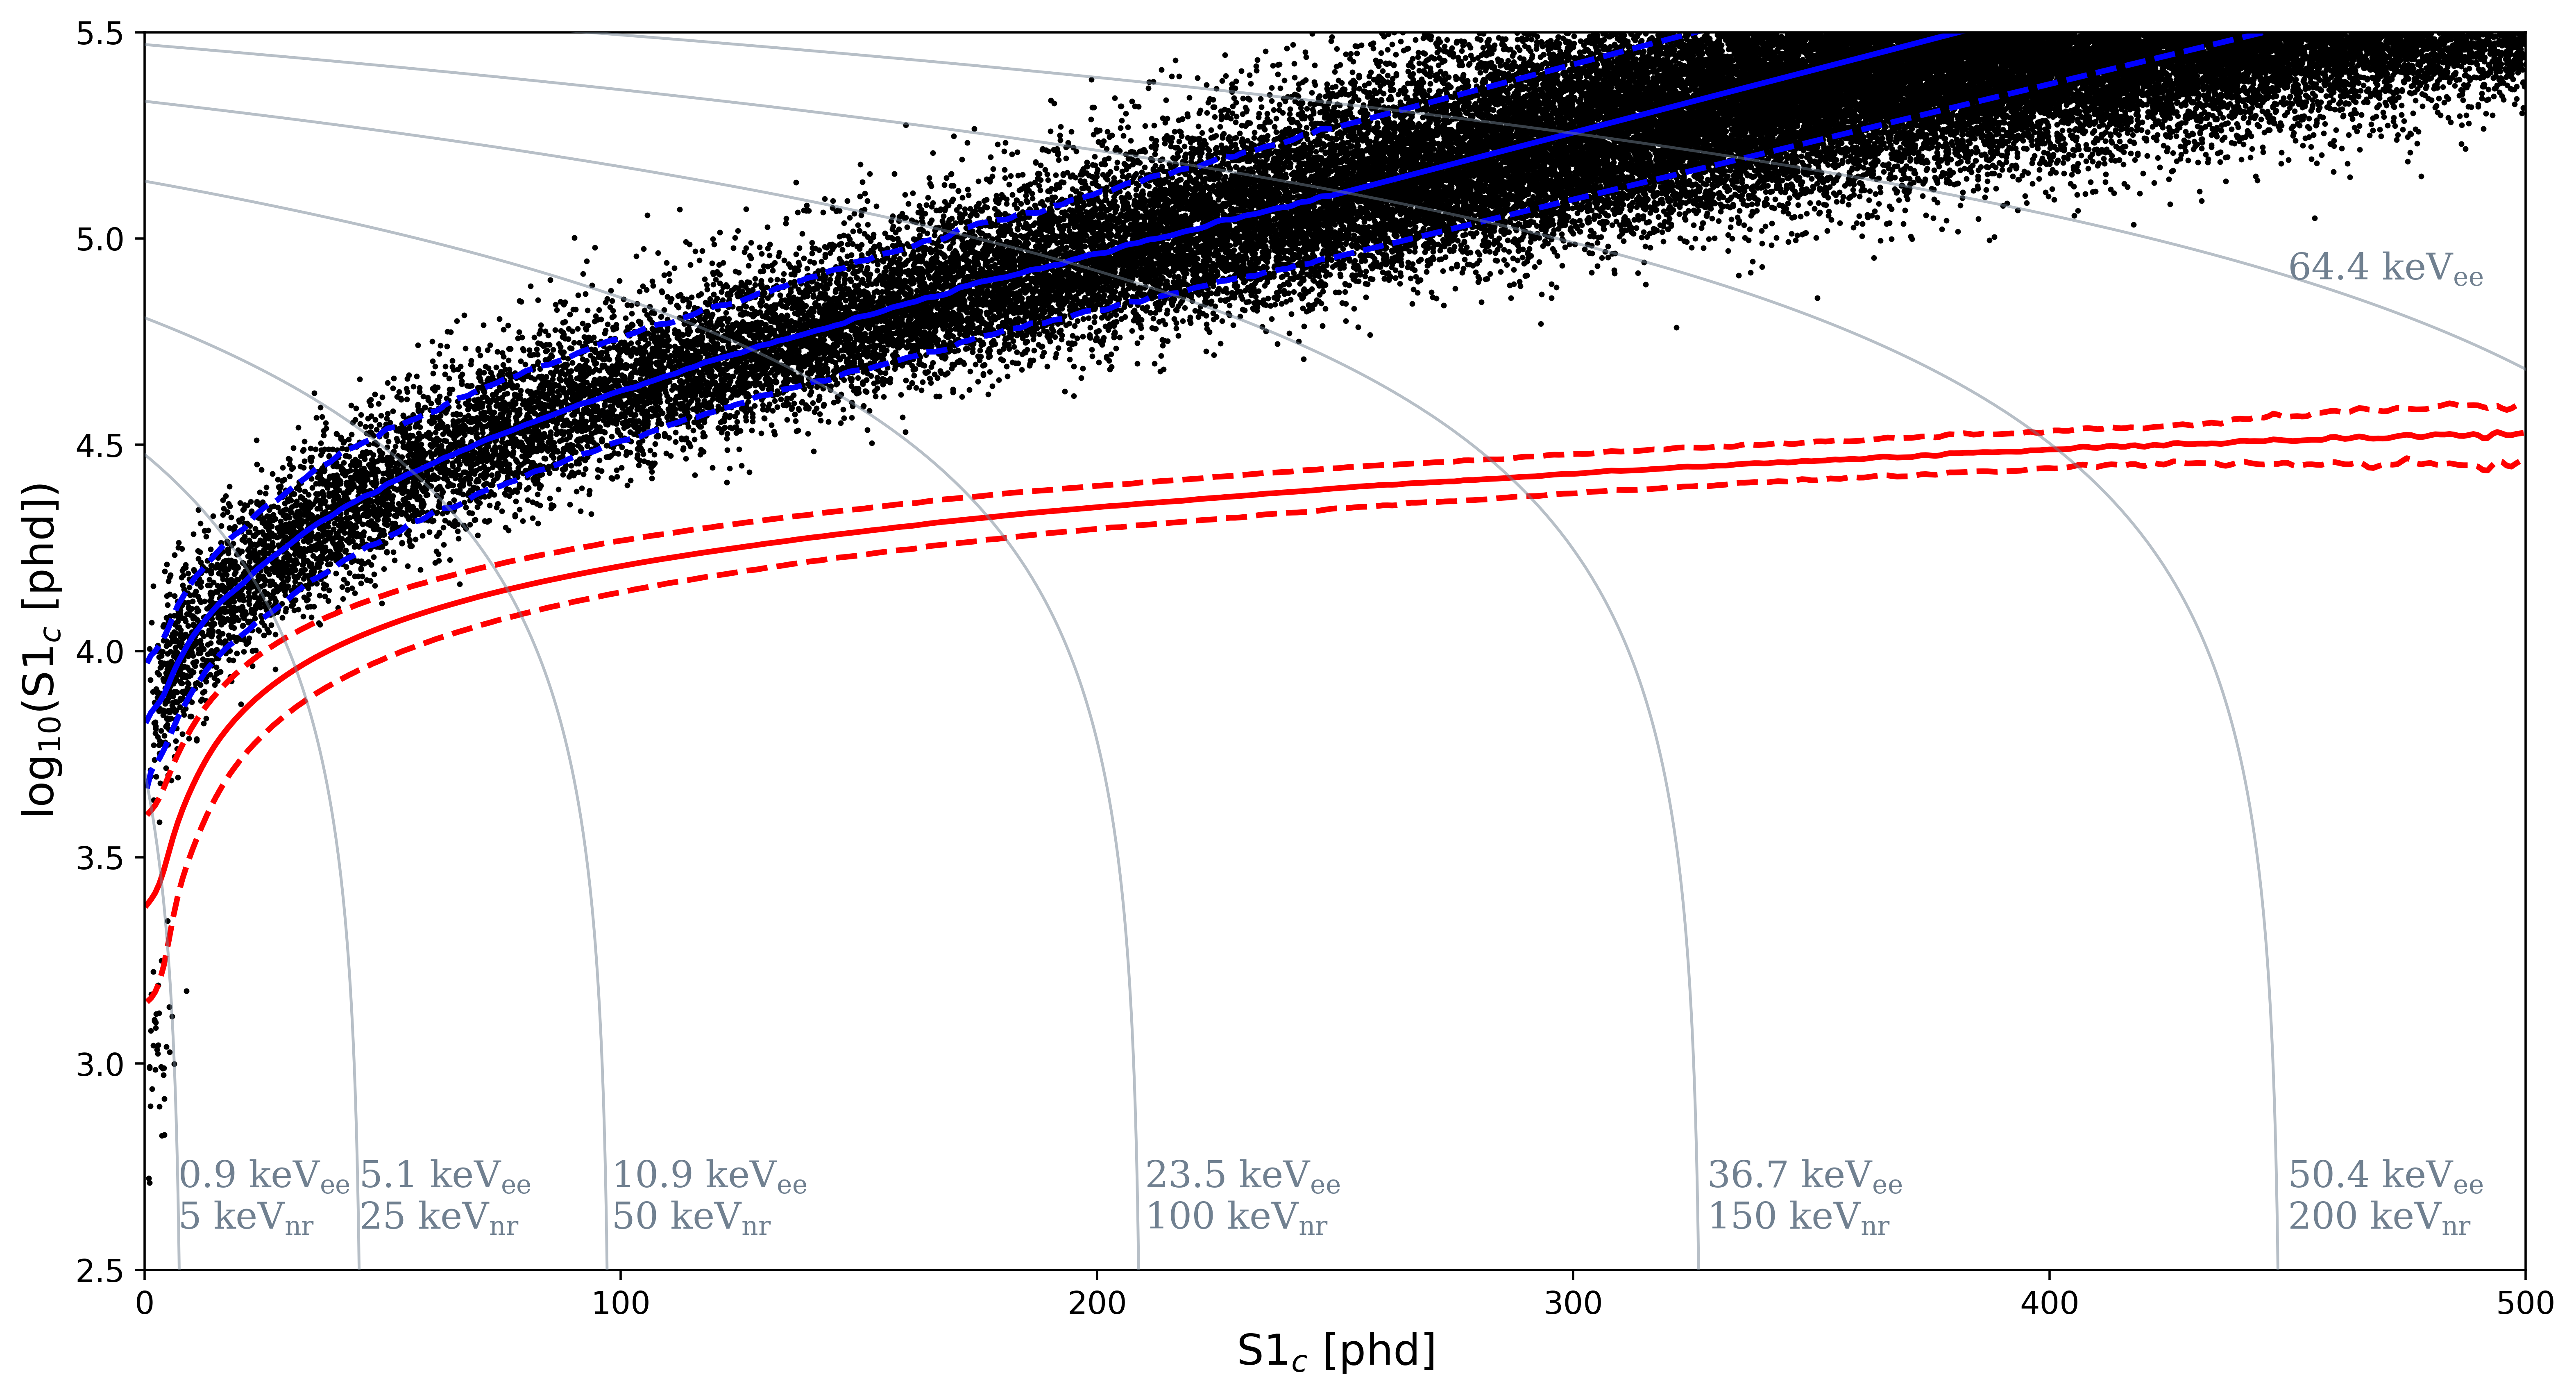
\includegraphics[width=15cm]{Figures/EFT/Projected_backgrounds/projected_backgrounds_s1_s2.png}
    \caption{Simulated data set for a background-only 1000 live day run with a 5.6 tonne fiducial mass. The ER and NR bands are shown in blue and red respectively; the solid lines are the mean and the dashed are 10\% and 90\% quantiles.}
    \label{fig:my_label}
\end{figure}





\subsection{Limits}
\par
A one-sided PLR test statistic was used in order to maintain software compatibility with these legacy simulations which were the basis of \cite{LZ_projected_sensitivity_paper_ref}.
The upper limits are shown in \autoref{fig:EFT_Result_Projected_Sensitivity_1} and \autoref{EFT_Result_Projected_Sensitivity_2}.
Note that the limit is presented in terms of the dimensionless values $({c}^{s}_{i}\times{m}^{2}_{w})^{2}$ rather than just $({c}^{s}_{i}$ (which has dimensionality of [mass]$^{-2}$, where $m_w$ is the Higg's vacuum expectation value.
This decision has been made due to several experiments making the decision to present them in this way (starting with XENON100 \cite{xenon100_eft_ref}).
\par
A key benefit of presenting in this manor is that it allows for a direct comparison to previous results which have been included in the limits shown.
Only a single data point is shown from LUX as their analysis was originally done in an \{$n,p$\} basis \cite{LUX_RUN4_EFT_2021}, and given the huge quantity of work it took they decided to reduce the problem to a single WIMP mass per operator.
\par
LZ has the potential to make significant strides in this region of parameter space which can be interpreted as 

\begin{figure}[!htbp]%
\centering
\begin{tikzpicture}
\centering
  \begin{groupplot}[view={0}{90},
    group style = {group size = 2 by 4,
                   vertical sep=1.5cm,
                   horizontal sep=2.0cm}]
    
    \pgfplotsforeachungrouped \x in {1,3,4,5,6,7,8,9}{
     \edef\tmp{
        \noexpand \nextgroupplot[
                                xlabel=Mass (MeV),
                                ylabel=$({c}^{s}_{\x}\times{m}^{2}_{w})^{2}$,
                                mark size=0pt,
                                width=0.45\textwidth,
                                height=5.5cm,
                                xmode=log,
                                ymode=log,
                                yminorticks=true,
                                x label style={at={(axis description cs:0.75,-0.1)},anchor=near ticklabel},
                                y label style={at={(axis description cs:-0.13,.75)},anchor=near ticklabel},
                                ]
            
            \noexpand \addplot[blue, name path = xenon100] table[]
                      {Data/HENR/Xenon100/O\x.dat};
                        
            \noexpand \addplot[only marks, mark size=1, error bars/.cd,
                               y dir=both, y explicit, error bar style={color=black}]
                               table[x=mass,y=median, y error plus index=3, y error minus index=2] {Data/HENR/Projected_Sensitivity/LUX/O\x.dat};
            
            \noexpand \addplot[green, opacity = 0.4, name path = nsig1] table[x=mass, y=nsig1]
                      {Data/HENR/Projected_Sensitivity/Results_method1/O\x.dat};
                      
            \noexpand \addplot[green, opacity = 0.4, name path = psig1] table[x=mass, y=psig1]
                      {Data/HENR/Projected_Sensitivity/Results_method1/O\x.dat};
                      
            \noexpand \addplot[yellow, opacity = 0.4, name path = psig2] table[x=mass, y=psig2]
                      {Data/HENR/Projected_Sensitivity/Results_method1/O\x.dat};
                      
            \noexpand \addplot[green, opacity = 0.4, forget plot] fill between[of=nsig1 and psig1];
            \noexpand \addplot[yellow, opacity = 0.4, forget plot] fill between[of=psig1 and psig2];
            
            \noexpand \addplot[black, name path = median] table[x=mass, y=median]
                      {Data/HENR/Projected_Sensitivity/Results_method1/O\x.dat};
            
            %\noexpand \addplot[black, dashed, name path = median] table[x=mass, y=cl]
            %          {Data/HENR/Projected_Sensitivity/Results/O\x.dat};
                     
        }
        \tmp 
        }
  \end{groupplot}
\end{tikzpicture}
\caption{}
\label{fig:EFT_Result_Projected_Sensitivity_1}
\end{figure}



\begin{figure}[!htbp]%
\centering
\begin{tikzpicture}
\centering
  \begin{groupplot}[view={0}{90},
    group style = {group size = 2 by 3,
                   vertical sep=1.5cm,
                   horizontal sep=2.0cm}]
    
    \pgfplotsforeachungrouped \x in {10,11,12,13,14,15}{
     \edef\tmp{
        \noexpand \nextgroupplot[
                                xlabel=Mass (MeV),
                                ylabel=$({c}^{s}_{\x}\times{m}^{2}_{w})^{2}$,
                                mark size=0pt,
                                width=0.45\textwidth,
                                height=5.5cm,
                                xmode=log,
                                ymode=log,
                                x label style={at={(axis description cs:0.75,-0.1)},anchor=near ticklabel},
                                y label style={at={(axis description cs:-0.13,.75)},anchor=near ticklabel},
                                ]
            
            \noexpand \addplot[blue, name path = xenon100] table[]
                      {Data/HENR/Xenon100/O\x.dat};
            
            \noexpand \addplot[only marks, mark size=1, error bars/.cd,
                               y dir=both, y explicit, error bar style={color=black}]
                               table[x=mass,y=median, y error plus index=3, y error minus index=2] {Data/HENR/Projected_Sensitivity/LUX/O\x.dat};
                        
            \noexpand \addplot[green, opacity = 0.4, name path = nsig1] table[x=mass, y=nsig1]
                      {Data/HENR/Projected_Sensitivity/Results_method1/O\x.dat};
                      
            \noexpand \addplot[green, opacity = 0.4, name path = psig1] table[x=mass, y=psig1]
                      {Data/HENR/Projected_Sensitivity/Results_method1/O\x.dat};
                      
            \noexpand \addplot[yellow, opacity = 0.4, name path = psig2] table[x=mass, y=psig2]
                      {Data/HENR/Projected_Sensitivity/Results_method1/O\x.dat};
                      
            \noexpand \addplot[green, opacity = 0.4, forget plot] fill between[of=nsig1 and psig1];
            \noexpand \addplot[yellow, opacity = 0.4, forget plot] fill between[of=psig1 and psig2];
            
            \noexpand \addplot[black, name path = median] table[x=mass, y=median]
                      {Data/HENR/Projected_Sensitivity/Results_method1/O\x.dat};
            
            %\noexpand \addplot[black, dashed, name path = median] table[x=mass, y=cl]
            %          {Data/HENR/Projected_Sensitivity/Results/O\x.dat};
                     
        }
        \tmp 
        }
  \end{groupplot}
\end{tikzpicture}
\caption{}
\label{fig:EFT_Result_Projected_Sensitivity}
\end{figure}
